\documentclass[twoside, headsepline, 12pt, a4paper, chapterprefix, bibtotoc]{article}

\newcommand{\HRule}{\rule{\linewidth}{0.5mm}}
\usepackage{array}
\usepackage{subfigure}
\usepackage{times}
\usepackage{url}
\usepackage{lscape}
\usepackage{natbib}
\usepackage{color}
\usepackage{wrapfig}
\usepackage[table]{xcolor}
\usepackage[final]{pdfpages}
\usepackage{ucs}
\usepackage{listings}
\usepackage{subfigure}
\usepackage{multirow}
\usepackage{float}
\usepackage{framed,lipsum}
\usepackage[utf8]{inputenc}
\usepackage[pdftex]{graphicx}


\usepackage[pdftex, pdfauthor={Karoly Szanto, Morten Esbensen},
pdftitle={Realms Project}, linkcolor=black, urlcolor=black,
citecolor=black, bookmarks=true, bookmarksopen=true, bookmarksnumbered=true, colorlinks=true, plainpages=false, pdfpagelabels]{hyperref}

\RequirePackage{color,graphicx}

%Setup hyperref package, and colours for links
\usepackage{hyperref}
\definecolor{linkcolour}{rgb}{0,0.2,0.6}
\hypersetup{colorlinks,breaklinks,urlcolor=linkcolour, linkcolor=linkcolour}

\newcommand{\todo}[1]{\textsf{\textbf{\textcolor{Orange}{[[#1]]}}}}
\newcommand{\myjavalisting}[0]{
\lstset{captionpos=b,language=java,numbers=none,basicstyle=\small}
\lstset{linewidth=1.0\textwidth}
\lstset{
keywordstyle=\bfseries\ttfamily\color[rgb]{0,0,1},
identifierstyle=\ttfamily,
commentstyle=\color[rgb]{0.133,0.545,0.133},
stringstyle=\ttfamily\color[rgb]{0.627,0.126,0.941},
showstringspaces=false,
basicstyle=\small,
numbers=none,
stepnumber=1,
numbersep=10pt,
tabsize=2,
frame=trbl,
breaklines=true,
prebreak = \raisebox{0ex}[0ex][0ex]{\ensuremath{\hookleftarrow}},
breakatwhitespace=false,
aboveskip={1.5\baselineskip},
columns=fixed,
upquote=true,
extendedchars=true,
}}
\newcommand{\myxmllisting}[0]{
\lstset{captionpos=b,language=xml,numbers=none,basicstyle=\small}
\lstset{linewidth=1.0\textwidth}
\lstset{
keywordstyle=\bfseries\ttfamily\color[rgb]{0,0,1},
identifierstyle=\ttfamily,
commentstyle=\color[rgb]{0.133,0.545,0.133},
stringstyle=\ttfamily\color[rgb]{0.627,0.126,0.941},
showstringspaces=false,
basicstyle=\small,
numbers=none,
stepnumber=1,
numbersep=10pt,
tabsize=2,
frame=trbl,
breaklines=true,
prebreak = \raisebox{0ex}[0ex][0ex]{\ensuremath{\hookleftarrow}},
breakatwhitespace=false,
aboveskip={1.5\baselineskip},
columns=fixed,
upquote=true,
extendedchars=true,
}}

\begin{document}

\pagestyle{empty}

\begin{titlepage}

\begin{center}


% Upper part of the page

\includegraphics[width=0.15\textwidth]{./fig/itu_logo}\\[1cm]    

\textsc{\LARGE IT-University of Copenhagen}\\[2.0cm]

% Title
\HRule \\[0.4cm]
{ \huge \bfseries Realms Project}\\[0.4cm]

\HRule \\[1.5cm]

% Author and supervisor
\begin{minipage}{0.4\textwidth}
\begin{flushleft} \large
\emph{Authors:}\\
K\'aroly Sz\'ant\'o\\
Morten Esbensen\\
\end{flushleft}
\end{minipage}
\begin{minipage}{0.4\textwidth}
\begin{flushright} \large
\emph{E-Mail:} \\
\href{mailto:ksza@itu.dk}{ksza@itu.dk}\\
\href{mailto:mortenq@itu.dk}{mortenq@itu.dk}\\
\end{flushright}
\end{minipage}\\[0.8cm]

% Author and supervisor
\begin{minipage}{0.4\textwidth}
\begin{flushleft} \large
\emph{Supervisor:}\\
Thomas Pederson\\
\end{flushleft}
\end{minipage}
\begin{minipage}{0.4\textwidth}
\begin{flushright} \large
\emph{E-Mail:} \\
\href{mailto:tped@itu.dk}{tped@itu.dk}\\
\end{flushright}
\end{minipage}

\vfill

% Bottom of the page
{\large \today}

\end{center}

\end{titlepage}
\cleardoublepage

\begin{abstract}
	\noindent With the rise in numbers of smart phones equipped with location-sensing technologies, location-based applications have become increasingly popular and are found in large numbers around the mobile phone application marketplaces. Location-based applications use the physical location of the user to allow for new ways of interacting with software or with other people.
\\\\
To further push location-based systems in to every day use, we present an end-user programming system - Realms - that allows users to augment physical locations with digital information. With Realms, users can augment physical locations with information through a web-interface centered around a simple map. The information is thereafter made available on the mobile phone application depending on basic rules and the behavior of the mobile phone user
\\\\
We describe our motivations, design rationale and implementation of the system and present a preliminary evaluation based on a test with 9 users. This evaluation showed that the participants found the system useful and easy to use and pointed to work on push-based communication and a more visual mobile client.
\end{abstract}

\newpage
% TOC
\setcounter{tocdepth}{3}
\tableofcontents

%\listoffigures
%\listoftables
\cleardoublepage

\pagestyle{plain}

%!TEX root = /Users/mortenq/Documents/ITU/Master/Realms/svn/itu_realms_project/trunk/realms_report/dk.itu.realms.main.tex
%I am structuring the introduction according to this guide: http://pages.cpsc.ucalgary.ca/~saul/wiki/pmwiki.php/Chapter1/Deconstruction. It's Saul Greenbarg's guide to thesis chapter 1's, but I think it works fine for smaller projects as well. If we find that the structure doesnt work we can always chagen it, but for now I think its a good way to do it (as it forces me think about every aspect)

%I've written something down. We probably need to re-write a lot of it till it sounds good
\section{Introduction}
\label{sec.introduction}
With the explosion of location-aware devices in the forms of mobile phones and tablets, location-based systems have become a reality rather than a vision. Programmers have many ways of using the location capabilities of these devices and numerous location aware applications are available for download. A lot of the systems are based on the same principles of basic context-awareness; the selection of available functionality or information, based on the context (location). However, despite the similarities of location-aware programs, developers needs to start from scratch when creating a new one. 
\\\\
In this project we want to explore the if it is possible to abstract the creation of simple location-based systems from a programming level to a configuration level.


\subsection{Motivation} % (fold)
\label{sub:context_and_motivation}
The use of location based systems have risen greatly over the last few years with the introduction of portable locatable devices. Location-based systems demonstrate a successful implementation of context-awareness and the popularity of systems such as foursquare and Facebook places shows that users have adapted this form of interaction. Companies as well use location information to a great extend, and meanwhile the process of programming location-aware application has become easy for programmers. Operating system and library support for obtaining location data now exists on most mobile platforms, and a few lines of code can yield a precise latitude and longitude of a device. Yet, programming experience is needed even to design the most simple location-based interaction. Holloway and Julien argue that for ubiquitous computing systems to become fully realized in the everyday environment, end-user programming must be available to bridge the gap between system and user \cite{Holloway:2010:CEP:1882362.1882398}. This will also serve as our motivation; to empower end users with the ability to augment physical locations with digital information in a simple non-programming way.
% subsection context_and_motivation (end)'

\subsection{Related Work} % (fold)
\label{sub:background}
This subsection should in short list related works in the area. We will write this we we have investigated the subject further.

% subsection background (end)

\subsection{Hypothesis} % (fold)
\label{sub:hypothesis}
It is our hypothesis that some common features of location-based systems can be identified, and that these features can be supported by a system designed to create location-based interaction. We want to develop a software infrastructure that, when configured, augments a certain physical area with digital capabilities. To elaborate, we introduce the notion of 'Realms'. A realm is a physically confined space augmented with digital information. A realm is always associated with a physical space, however it can provide different affordances; a game, a campaign, general public information etc. Access to the realms is provided through a mobile phone application, and so only one app is needed to access any number of realms with any number of affordances. The managing of realms is handled by a server that phones connect to and the creation of realms is handled through a web-interface. 
% subsection hypothesis (end)

\subsection{Goals and Methods} % (fold)
\label{sub:goals_and_methods}
Our goals with this project are three-fold:

\begin{enumerate}
	\item We will investigate popular location based apps and factor our the commonalities. From this investigation we will present a 
	\item We will implement a Realms system that allows for the creation of augmented physical spaces through configuration. 
	\item We will present an evaluation of the system and discuss it's possibilities and limitations
\end{enumerate}

\noindent To reach these goals, we will take the following steps:

\begin{enumerate}
	\item  We will study a number of popular location-based applications and group their functionalities. 
	\item We will use the study of existing apps to select a few key functionalities that are popular in location based apps. We will build the Realms system to support these findings.
	\item We will evaluate our system in two ways; (1) we will have users try the configuration manager to study the effectiveness and ease of use of our system, and (2) we will compare the functionalities of our system to those found in our study of other systems to conclude on the possibilities and limitations of our system.
\end{enumerate}
% subsection goals_and_methods (end)

\subsection{Contributions} % (fold)
\label{sub:contributions}
Our main contributions follow our goals:

\begin{itemize}
	\item We present a taxonomy for location-based application functionalities. 
	\item We present the Realms system. A software platform for augmenting physical locations through configuration.
	\item We present an discussion of the feasibility of our implementation based on a user evaluation.
\end{itemize}
% subsection contributions (end)

\subsection{Overview} % (fold)
\label{sub:overview}
The remainder of the report is structured as follows. In section we present related work on augmented spaces and end user programming. In section 3 we analyze existing location-based apps as well as app creation systems. We focus on drawing out similarities between the systems and present a taxonomy of location application functionalities. We then, in section 4 present our design rationale for the Realms system, and present the implementation details in section 5. In section 6 we present our evaluation of the system and and follow with a discussion of the results in section 7. We end in section 8 by concluding and suggesting directions for future work in the area.
% subsection overview (end)

\clearpage
\section{Related Work} % (fold)
\label{sec:related_work}
This section will contain related work

\subsection{Agumented Spaces} % (fold)
\label{sub:agumented_spaces}
The main functionality of our proposed system is the ability to create augmented physical spaces. In this subsection we will explore related works on augmented spaces. A very interesting field is location based games as described in the research literature.
% subsection agumented_spaces (end)

\subsection{End user programming} % (fold)
\label{sub:end_user_programming}
The method for creating realms is trough configuration rather than programming - therefore end user programming becomes an interesting field to study as well.
% subsection end_user_programming (end)
% section related_work (end)
\clearpage
%!TEX root = /Users/mortenq/Documents/ITU/Master/Realms/svn/itu_realms_project/trunk/realms_report/dk.itu.realms.main.tex
\section{Analysis} % (fold)
\label{sec:analysis}
To gain a better understanding of the type of system we are developing, there are a number of fields we need to explore. Our system will allow users to create Realms - that is digitally enhanced physical locations. The motivation behind our system is the ability to allow end-users to configure these types of interactions. Having described related work in the fields of location-based system and end-user configuration for context-aware computing, we identify two important fields that we will analyze before we proceed; an abstract view on location based systems and the concept of Realms.

\subsection{Characterization of Location Based Systems} % (fold)
\label{sub:taxanomy_of_location_features}
In this subsection we will try to characterize the properties of location-based systems. To do so we list a number of design dimensions that each describe a property of a location based systems. It is worth noticing that most location-based systems employ several features that does not have anything to do with location. While the foundations of the system may be dependent on location data, a lot of functionality that uses the location data in clever ways are supported. The design dimension we mention here are concerned only with interaction that are location-based. 

\subsubsection{Location Representation}
When we talk about location, we talk about the physical location of a user in the world. It is however important to notice that location can be represented in different ways. In general we can express location in 3 different ways; absolute, symbolic and relative (ref ubicomp book). The absolute location is the location expressed in the absolute measurements as defined by the system. For the earth as our system, the absolute location measurement is a position expressed in terms of latitude and longitude. The symbolic location measurement is a measurement that is meaningful to an interpreter (such as a human). An example would be The university - a location that makes sense for students and employees. Lastly location can be expressed in terms of relative position - that is, a position relative to another- for example 2 kilometers north of Copenhagen (note that Copenhagen is a symbolic location in this example).

\subsubsection{Location Level}
Location type describes the characteristics of the location information used in an interaction. We define two distinct levels to which location systems make use of location information; location-based and location-enhanced. The location-based are interaction in which the outcome or result of the interaction depends on the location of the user. A good example is a search for nearby restaurants using a mobile location-enabled device. The search results from e.g. Google Search, will depend on the location of the user and their sorting likewise. On the other hand, location enhanced interactions are those where location is used to augment an interaction without affecting the outcome of it. An example is a check-in on e.g. Facebook Places. This outcome of the interaction is the check-in of the user - regardless of his location though his location is recorded. Later, a series of location based interactions may occur that follow the location-enhanced one, e.g. if a user want to search for other people in the vicinity using his previously reported location.

\subsubsection{Data Type}
The data type is a dimension we we adopt from Schilit et. al.'s categorization of context aware computing applications \cite{512740}. For data type we distinguish between information and commands. Information is data as information distributed within the system. Commands on the other hand, are executed within the systems. Again, a Goole search for restaurants will return what we characterize as information; a list of restaurants. On the other hand, presenting the user with the ability to print at a nerby printer, or allowing a check-in at a given location is a location-based command.

\subsubsection{Communication Type}
Our last dimension is the communication type. This dimension describes whether a user should query the system for updates or whether this happens automatically. An example of the fist one is the, again, a search where a user queries the system for some search results. On the other hand, a system notifying a user when he's close to a given location is an automatic system.  

% subsection taxanomy_of_location_features (end)


\subsection{Design Space} % (fold)
\label{sub:design_space}
To sum up, we have identified 4 dimensions that can be use to characterize a location-based system. These are; location representation, location type, data type, communication type. Based on these dimensions we present our design space for location based systems.  \emph{Here we will have a picture with the design dimensions as a design space}
% subsection design_space (end) 


\subsection{Realms} % (fold)
\label{sub:realms}
We introduce the notion of \emph{Realms} to describe a physically confined place augmented with digital information accessible by our systems. This choice is not random but motivated by several factors. The definition of the word \emph{realm} is "A community or territory over which a sovereign rules; a kingdom."\footnote{\url{http://www.thefreedictionary.com/realm}}. This definition has inspired us to choose the word. A realm is in systems is not associated with a kingdom , but it does describe rules and affordances of a territory. The sovereign or kingdom in our system can thus be thought of as the rules of the realms as dictated by the person who configured it. 

Other uses of the word is found in online gaming - such as the online game World of Warcraft\footnote{\url{http://www.worldofwarcraft.com}} - where a realm is a synonym with an instance of the virtual world in which the game resides. This usage also fist will with our thoughts on realms. Indeed when entering a Realm in our system, the user is presented with a new virtual world.
% subsection realms (end)
% section analysis (end)



\clearpage
\section{Design} % (fold)
\label{sec:design}
This section will include our design ideas for the realms system

\subsection{Realms Infrastructure} % (fold)
\label{sub:realms_infrastructure}

% subsection realms_infrastructure (end)

\subsection{Configuration Manager} % (fold)
\label{sub:configuration_manager}

% subsection configuration_manager (end)

\subsection{Realms Android App} % (fold)
\label{sub:realms_android_app}

% subsection realms_android_app (end)
% section design (end)
\clearpage
\section{Implementation}
\label{sec.implementation}
\noindent The first step towards establishing the technologies which are most suited for this project, was to draw a high level architecture of the system. As the system is a lot about user interaction (i.e. presentation layer) we decided to go for a concrete separation between the domain~logic and the user~interface; the way to go in order to achieve this separation in a web application is by relying on the n-Tier architectural pattern. As we also need a persistent~storage which should also be separated by the domain-login and user-interface, we notice that our application is structured in to three layers. Hence, we are dealing with a system leveraging the 3-Tier\footnote{\url{http://en.wikipedia.org/wiki/Multitier_architecture}} architectural pattern, depicted in Figure\ref{fig.setup}.
\begin{figure}[H] 
	\centering
	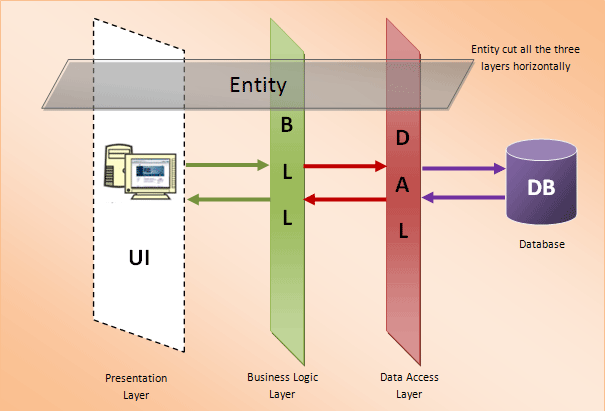
\includegraphics[width=\linewidth]{fig/3tier2}
	\caption{Concept of the 3-Tier Architectural pattern}
	\label{fig.setup}
\end{figure}
\\

\noindent Analysing the concept, we can see that it helps the application to separate the input~logic, business~logic and UI~logic, while providing a loose coupling between these elements. This allows for independent development, testing and maintenance of each component - called separation~of~concerns.
\\

\noindent Researching the frameworks that can help us carry out the current work, we have found a few suitable candidates: Apache~Struts\footnote{\url{http://struts.apache.org/}}, ASP.Net\footnote{\url{http://www.asp.net/}} and Java~Server~Faces (JSF)\footnote{\url{http://www.oracle.com/technetwork/java/javaee/javaserverfaces-139869.html}}. When choosing the framework to use, we had to take into consideration the following constraints:
\begin{itemize}
  \item the framework has to be free and open-source; free, because we do not
  have a budget to buy software and open-source because this is an academic
  project and we want to promote open-source
  \item we have an account on an ITU server to deploy the system; this
  server runs a Unix-like operating system; hence the framework should run on
  Unix-like platforms
\end{itemize}
\\

\noindent ASP.Net is a web application framework, developed by Microsoft. We have excluded this candidate because it fails to adhere to both constraints listed above; it is not open-source and runs only on the Microsoft Windows platform.
\\

\noindent Apache Struts is an open-source web application framework helping to develop Java EE web applications. It is based on the Java Servlet API, encouraging the use of MVC architecture. This framework satisfies both constraints, but it is a rather old technology, supporting Java~Server~Pages (JSP) for the presentation layer.
\\

\noindent We wanted to go for something more fresh, choosing JSF~2 as the framework to base our development upon. JSF is a Java-based web application framework which simplifies the development integration of web-based user interfaces. The core features, together with the help they offer for our development process, are listed bellow, as summarized by \cite{wiki}. We have leared the basics of JSF2 using \cite{Geary:3}.
\begin{itemize}
  \item managed beans (a dependency~injection system) -- helps to easily manage the creation and injection of objects the system depends upon
  \item built in ajax support -- useful for dynamic form validations
  \item integration with the Unified Expression Language (EL), which represent the core function of JSF; views may access managed bean fields and methods via EL
  \item a default set of HTML and web-application specific UI components -- to easily create good-looking and complex pages
  \item state management, supporting: "request'', "session'' and "application'' scoped Java beans -- helps to easily manage the lifetime of the managed beans.
\end{itemize}
\\

\noindent A JSF application needs to be deployed in an environment that is a web~server and which provides a servlet~container; although there are many options (JBoss, Glassfish etc.) we chose the simplest, Apache Tomcat 7, which is a lightweight open source web server and servlet container.
\\

\noindent Moreover, to build a robust and safe system in such a short period of time, we had to look for frameworks that can ease the development process in the main areas of the project: presentation, business and data access.

\paragraph{In the data access layer} the development can become a lot easier having entities (classes) representing equivalents of the tables in the database. This is an important aspect, as it is a lot easier to interact with the database in an Object-Oriented (OO) manner, from code written in an OO language, by invoking operations on objects, than to write queries against the database. For this purpose we chose Hibernate, which is an object-relational mapping (ORM) library for the Java language, providing a framework for mapping an object-oriented domain model to a traditional relational database.

\paragraph{In the business layer} the most important aspects are security, bean management and flow~control. We immediately found a potential candidate which soon proved to be the a very good one: the Spring Framework -- an open source application framework for the Java platform, providing the following modules which we used:
\begin{itemize}
  \item Inversion of Control container (Dependency injection) -- container which provides a consistent means of configuring and managing Java objects using reflection. The container is responsible for managing object life-cycles: creating objects, calling initialization methods, and configuring objects by wiring them together \cite{wiki_spring}. Therefore, we used the bean manager provided by this module to manage JSF, Hibernate and Spring beans.
  \item Data access framework (mostly in the data access layer) -- addresses common difficulties developers face when working with databases in applications, providing support for all popular data access frameworks in Java (JDBC, Hibernate etc.). Some of the  features made available by this module are: Resource management\footnote{automatically acquiring and releasing database resources}, Exception handling\footnote{translating data access related exception to a Spring data access hierarchy}, Transaction  participation\footnote{transparent participation in ongoing transactions}, Resource unwrapping\footnote{retrieving database objects from connection pool wrappers} \cite{wiki_spring}.
  \item Spring Security -- is a Java framework that provides authentication, authorization and other security features for enterprise applications.
\end{itemize}

\paragraph{In the presentation layer} in order to easily achieve a polished user interface we used \emph{PrimeFaces}\footnote{http://www.primefaces.org/} -- an open source JSF component library featuring a large number of components.

\noindent Summing up, our system is built upon JSF 2.1, using Hibernate 3.6 for ORM and Spring Framework 3 for bean management, data access and security while using MySQL 5 for a database. The system is deployed in Tomcat 7. Combining these technologies was also enforced by SpringSource presentation\cite{tomcat_spring}, which states that Tomcat and Spring are a perfect match.
\\

\subsection{Realms Configurator}
\noindent The most important aspect of the configurator is to provide the user with an easy to use and intuitive interface to easily place markers on physical locations. Most people using computers probably used or at least heard about \emph{Google Maps}\footnote{http://maps.google.com/}. We have decided to build our configurator on top of Google Maps, therefore the only previous knowledge to on how to navigate in google maps and how to place a marker on the map will help users create Realms and markers.
\\

\begin{figure}[H] 
	\centering
	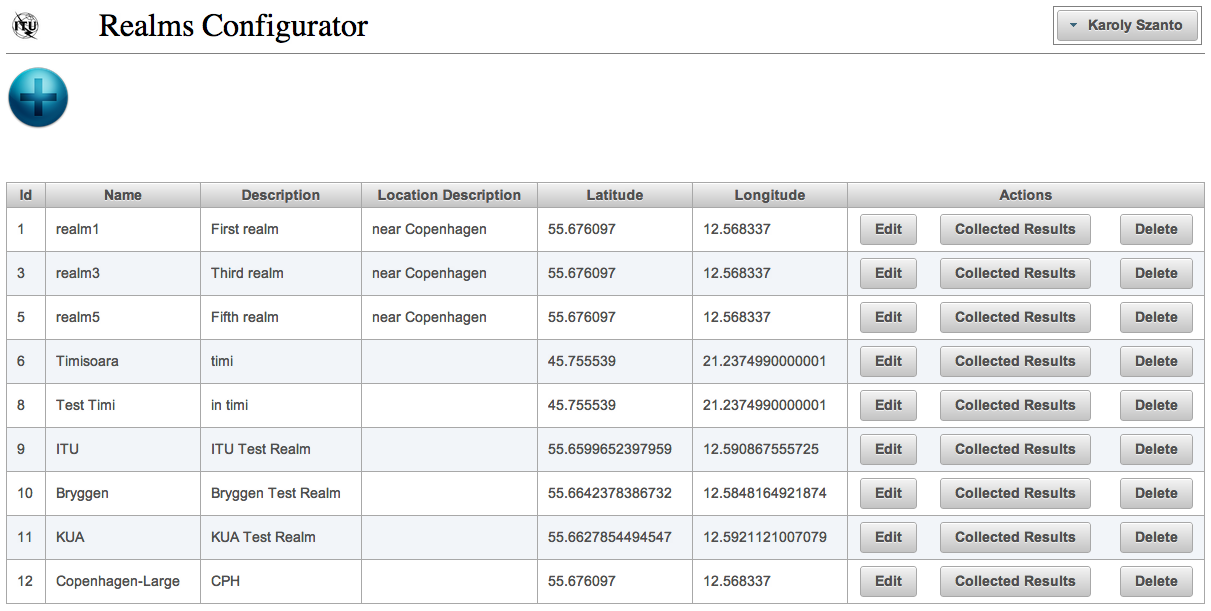
\includegraphics[width=\linewidth]{fig/my_realms.png}
	\caption{"My realms" view}
	\label{fig.my_realms}
\end{figure}

\noindent Figure \ref{fig.my_realms} depicts the home page of the configurator which presents the user with the realms he has created so far, if any. The user can choose to \emph{Create} (the "+" button) a new realm, to \emph{Edit/Delete} an existing one or to see the \emph{Collected Results} (presents the persisted realm users feedback -- answers to questions or ratings for informations).
\\

\noindent By pressing the create new realm button the user will be presented with the "Create Realm" page depicted in Figure \ref{fig.new_realm}. A search by address feature helps for easy navigation to the desired location described by a complete address, a city name, a symbolic location name (e.g IT University of Copenhagen) etc. To achieve the desired precision when placing the marker on the map, the user can use the zoom in and zoom out features to get a more/less detailed view and can drag the marker to another location. The radius of the realm (represented in meters) can be adjusted by modifying the appropriate input field. The realm radius is represented as a red circle around the marker. Once all the required data has been filled in, the user can save the newly created realm.
\begin{figure}[H] 
	\centering
	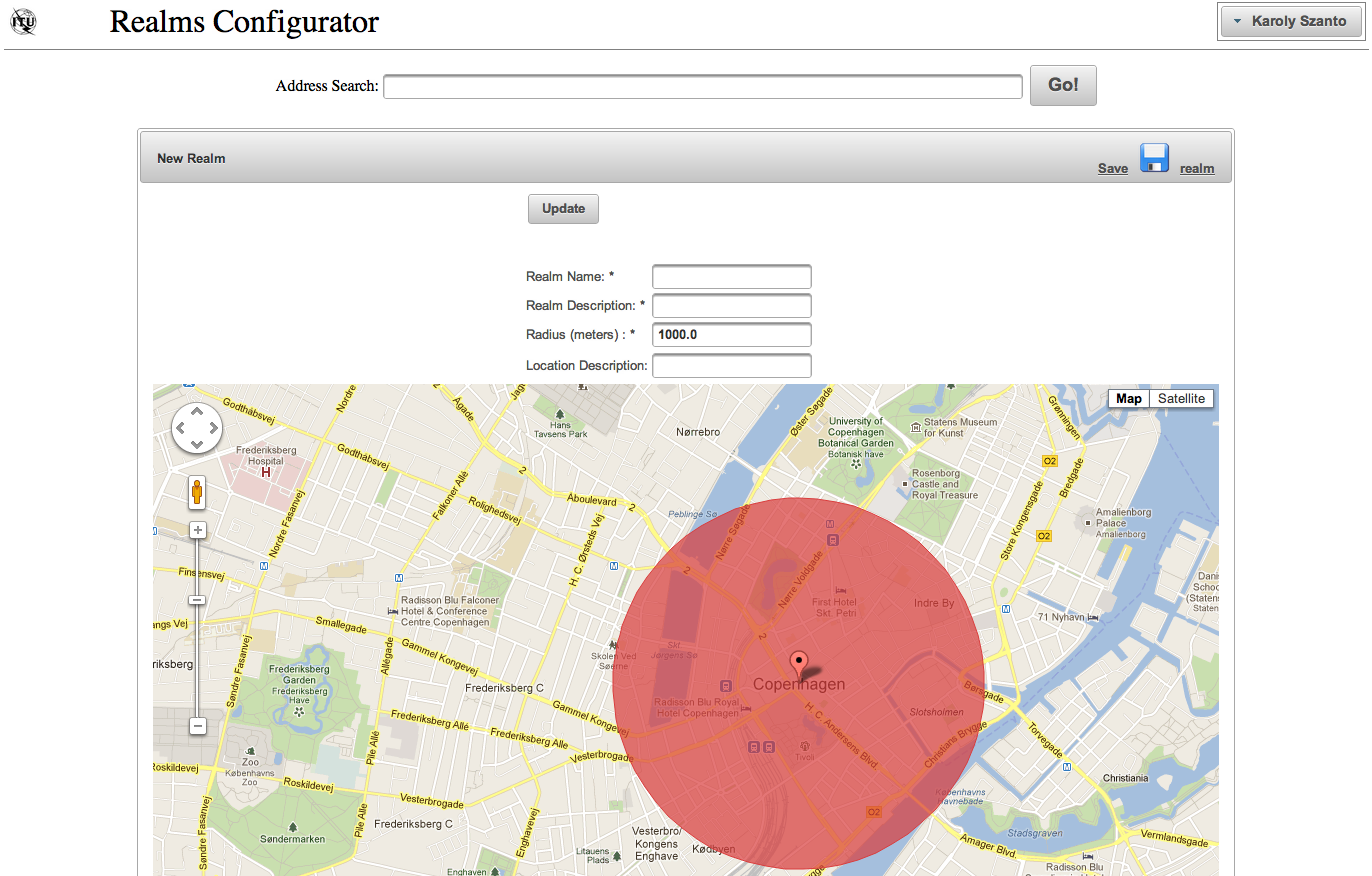
\includegraphics[width=\linewidth]{fig/new_realm.png}
	\caption{"Create Realm" view}
	\label{fig.new_realm}
\end{figure}
\\

\noindent Adding markers to a realm is supported in the "Configure Realm" page illustrated in Figure \ref{fig.edit_realm1}. This page can be reached either by saving a newly created realm in the create realm page or by choosing the edit realm option in the my\_realms page.
\begin{figure}[H] 
	\centering
	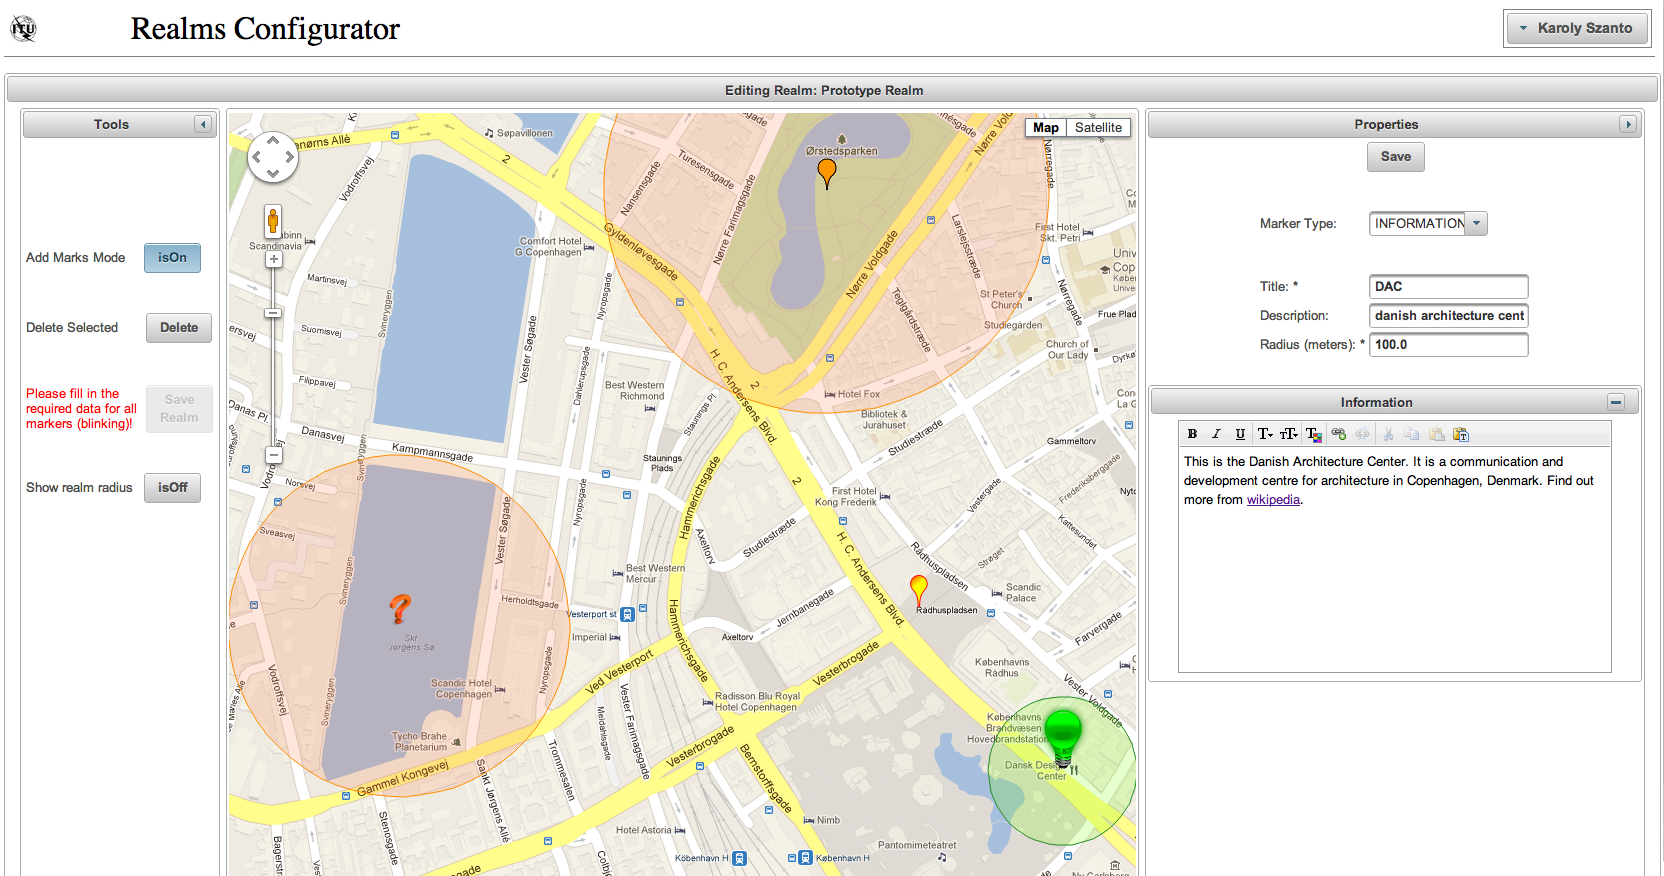
\includegraphics[width=\linewidth]{fig/edit_realm1.png}
	\caption{Edit Realm view with incomplete makers}
	\label{fig.edit_realm1}
\end{figure}
\noindent This page is made up by three different panes:
\begin{itemize}
	\item Tools -- the left pane provides general tools to help the configuration process
 	\item Map -- the central pane provides a map on which markers can be placed
	\item Properties -- the right pane allows editing the selected markers properties.
\end{itemize}

\noindent First we will describe each option provided by the tools pane:
\begin{itemize}
	\item Add marks mode -- enables or disables adding markers to the map. When this option is enabled, a simple click on the map will create add a new marker at that location.
	\item Delete selected -- deletes the selected marker. Only enabled if a marker is selected.
	\item Save realm -- save all the changes made so far and take the user back to the my\_realms page. This option is only enabled if all the required data for all the markers in the realms is filled in.
	\item Show realm radius -- toggle between displaying or hiding the circle representing the coverage area of this realm.
\end{itemize}

\noindent When markers are added to the map they don't have any data filled in by default. It is the users responsibility to configure each marker with the desired information. A marker can be configured as either information or a question. Therefore, a marker can be in different states during a configuration process which requires different graphical representations to make the interaction intuitive and easy:
\begin{itemize}
	\item a marker that does not have all the required data filled in is represented as an inverted water drop with a blinking black dot in the middle
	\item an information marker is represented as a light bulb
	\item a question marker is represented as a question mark
	\item unselected markers are orange whereas the selected marker is green and double in size.
\end{itemize}

\noindent As mentioned before, the properties pane enables the user to edit the selected markers properties. The selected marker in Figure \ref{fig.edit_realm1} is configured to be an information marker (the required properties are title and radius). The information is typed into a an input element with rich text editing features. In Figure \ref{fig.edit_realm2} the selected marker is a question marker. The properties pane is slightly different -- instead of entering information the user can enter a question (in the same editor enabled with rich text editing features) together with a set of possible options to choose from. At most one of the options can be marked as an answer.
\begin{figure}[H] 
	\centering
	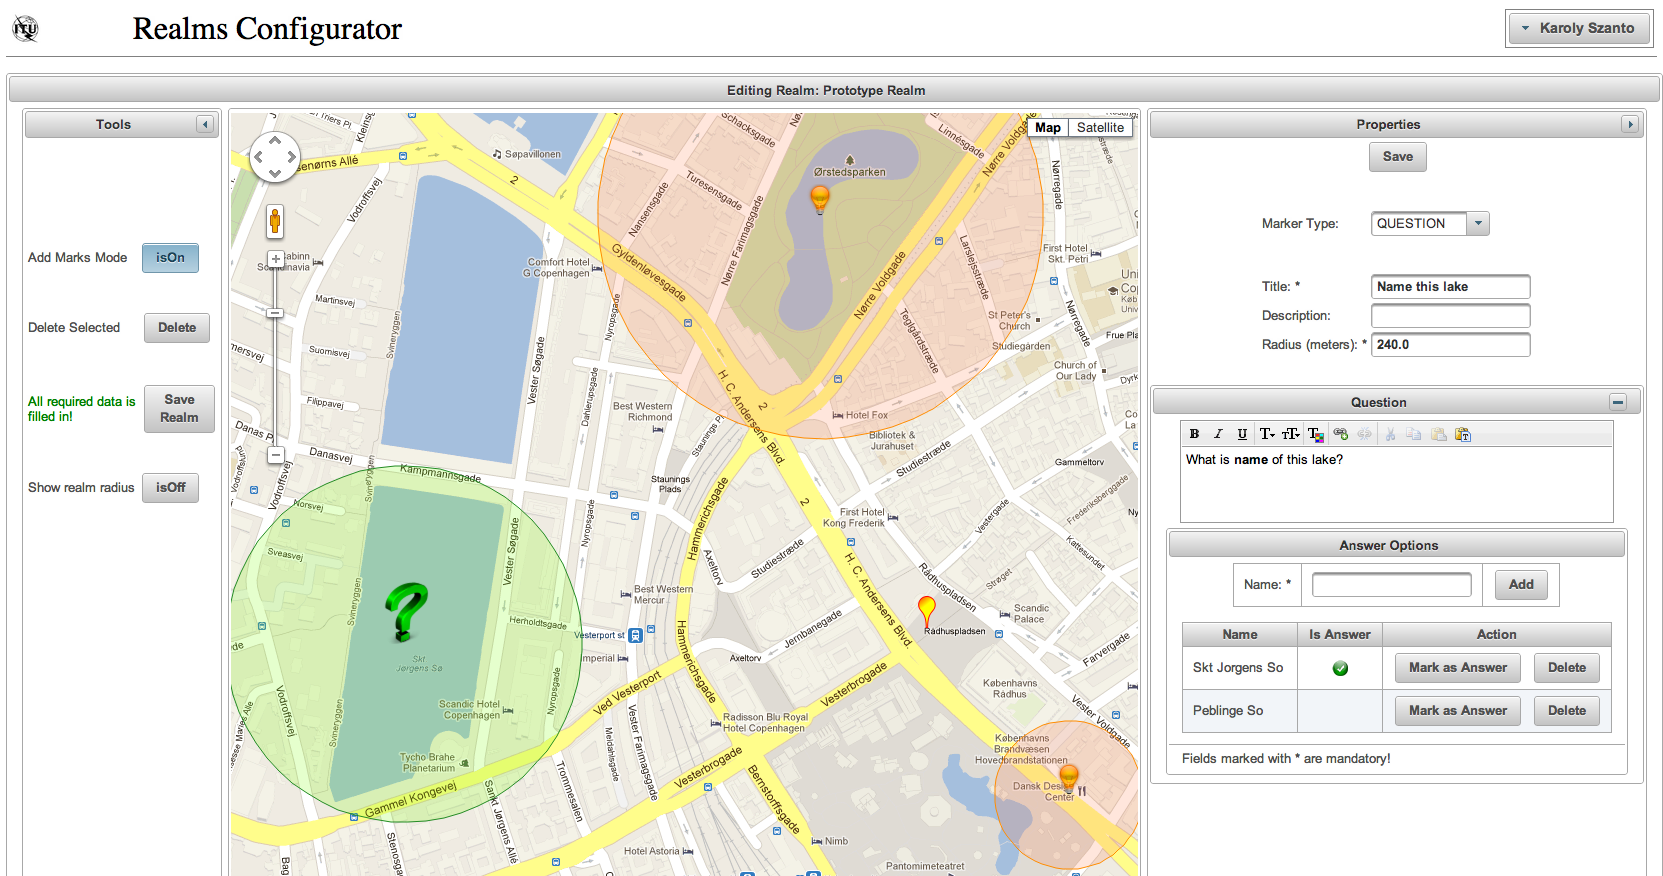
\includegraphics[width=\linewidth]{fig/edit_realm2.png}
	\caption{Edit Realm view with complete markers}
	\label{fig.edit_realm2}
\end{figure}

\noindent Finally, we would like to shortly describe the feedback page depicted in Figure \ref{fig.feedback} which presents the feedback collected from the realm users. As illustrated in the figure, each entry represents an individual feedback characterised by the user who submitted it, the marker it was submitted for, and the user feedback. For an information marker the feedback is a rating ranging from 1-5 and for a question marker it is the selected option (from the marker's set of possible options).
\begin{figure}[H] 
	\centering
	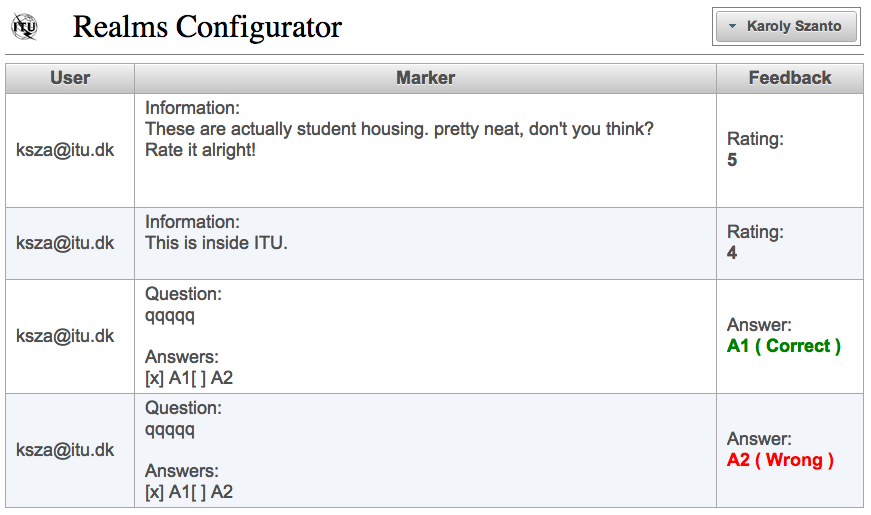
\includegraphics[width=\linewidth]{fig/feedback.png}
	\caption{Feedback page}
	\label{fig.feedback}
\end{figure}


\subsection{Realms Android App}
\noindent We have implemented the mobile client as an Android application. The application has to perform three main tasks:
\begin{itemize}
	\item provide the most accurate location as long as the application is running
	\item carry out location-based and location-enhanced interactions with the server
	\item present the user with the results of the interactions
\end{itemize}

\noindent For data sensing we have used the Funf Open Sensing Framework\footnote{http://funf.media.mit.edu}. The Funf Open Sensing Framework is an extensible sensing and data processing framework for mobile devices, developed at the MIT Media Lab. We have chosen this framework because it provides built-in accurate location sensing making use of GPS, Wi-Fi and mobile network (GPRS tower cell ID) data to accurately locate the device. At application start-up we start Funf's monitoring service. Each time we get a new reading, we store it in a local database. We have configured Funf to report location data sensed having an accuracy of at most 20 meters. This way the latest accurate location is available to be read by component of the application.
\\

\begin{figure}[H]
        \centering
        \subfigure[]{
                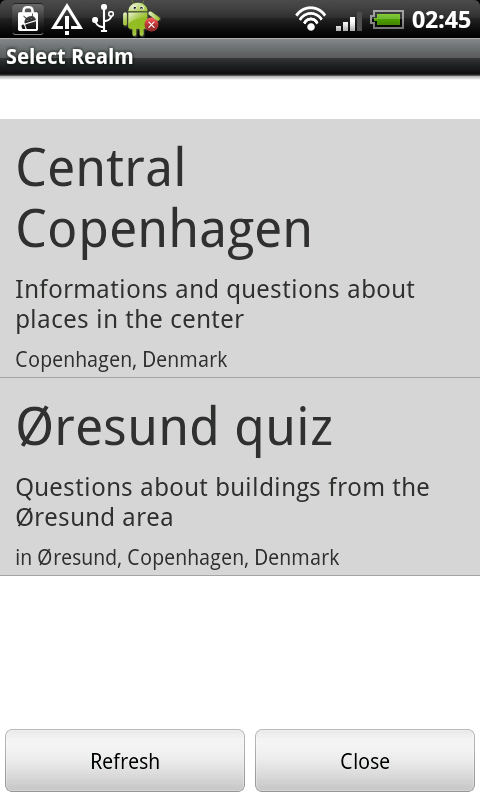
\includegraphics[width=0.3\linewidth]{fig/client/select_realm.png}
                \label{fig.client.select_realm}
        }
        \subfigure[]{
                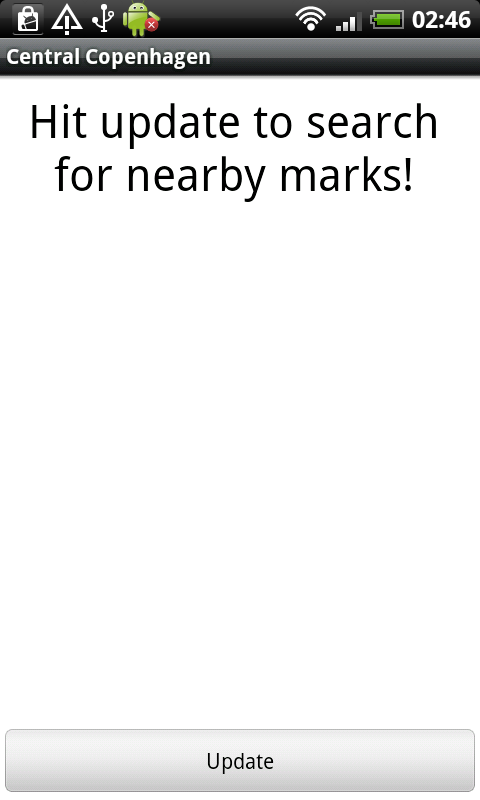
\includegraphics[width=0.3\linewidth]{fig/client/search_for_marks.png}
                \label{fig.client.find_markers}
        }
        \subfigure[]{
                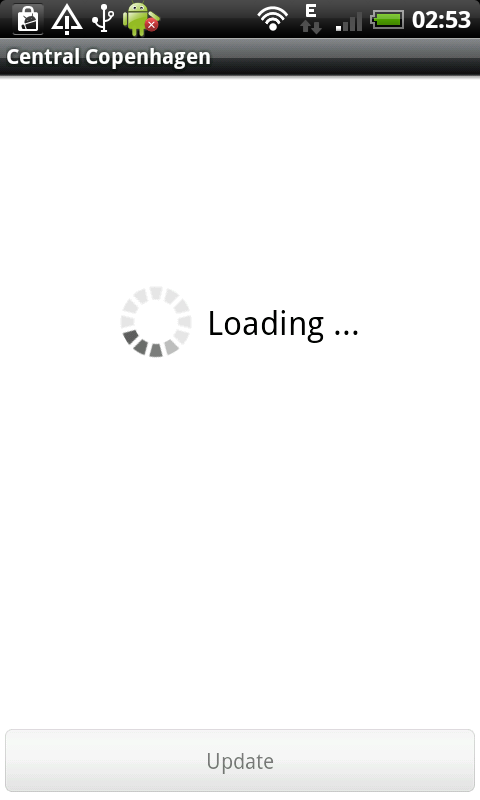
\includegraphics[width=0.3\linewidth]{fig/client/loading.png}
		\label{fig.client.loading}
        }
        \subfigure[]{
                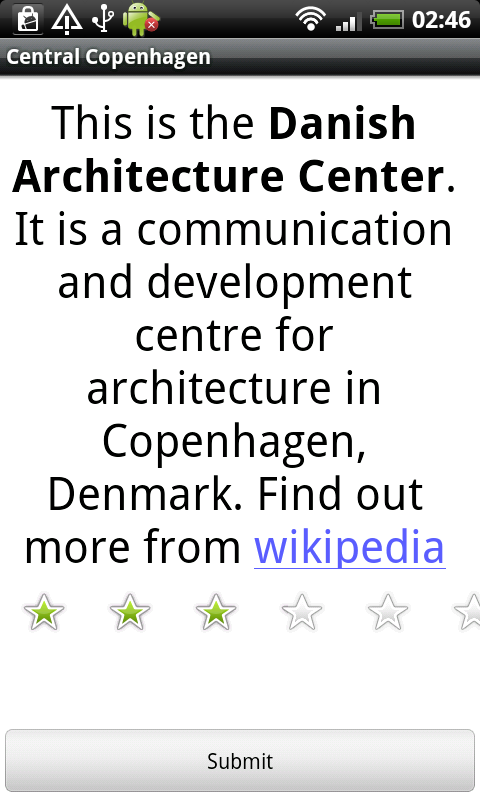
\includegraphics[width=0.3\linewidth]{fig/client/info_marker.png}
                \label{fig.client.info_marker}
        }
        \subfigure[]{
                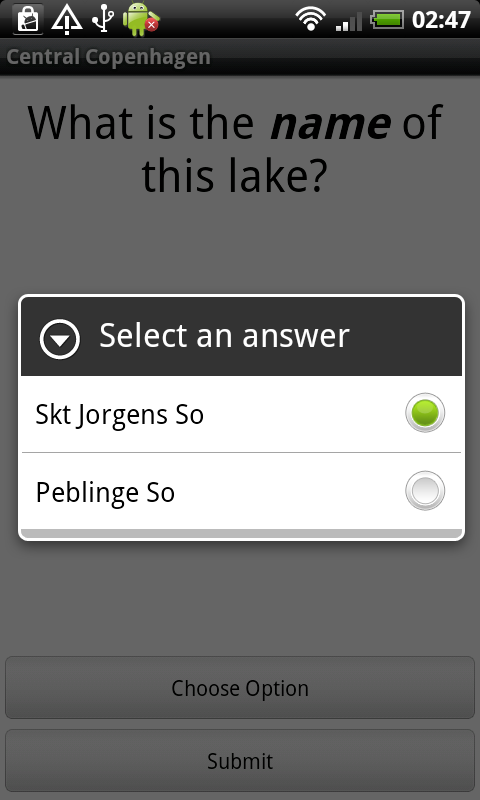
\includegraphics[width=0.3\linewidth]{fig/client/question_marker.png}
                \label{fig.client.question_marker}
        }
        \subfigure[]{
                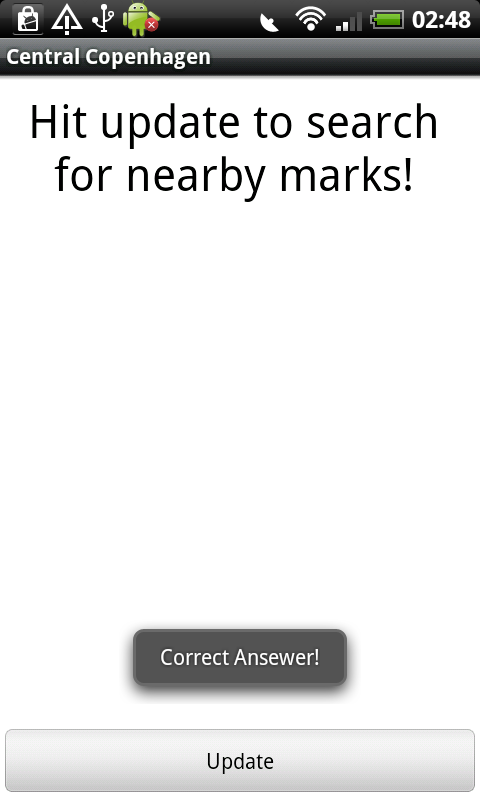
\includegraphics[width=0.3\linewidth]{fig/client/answer_feedback.png}
                \label{fig.client.answer_feedback}
        }
        \caption{The Realms Android App in action}
        \label{fig.client}
\end{figure}
\noindent Figure \ref{fig.client} depicts six screenshots of the working application which, in the followings, will help us discuss the implemented features. The first screen that is displayed to the user is the "select realm" screen illustrated in Figure \ref{fig.client.select_realm}. Once an accurate location reading is available, touching the refresh button will query the server for the realms the user is currently in. A list of realms might be returned (if any) and presented to the user. Choosing one of the realms will take the user to a screen which enables the user to search for markers in the selected realm. Therefore, as depicted in Figure \ref{fig.client.find_markers} the user can query the server for nearby markers clicking on the Update button. It has to be noted that each communication with the server is time consuming and the user has to be informed about this. Figure \ref{fig.client.loading} illustrates a loading screen which we used to inform the user about the long running operation every time a communication with the server is in process.
\\

\noindent After an update process the screen is populated with the marker data. For the information marker, illustrated in Figure \ref{fig.client.info_marker}, the formatted information data is displayed together with a rating bar rate the information in the marker. For the question marker, depicted in Figure \ref{fig.client.question_marker}, on the other hand, the screen displays the formatted question and a list of choices to choose an answer from. In both cases, information and question marker, a feedback will be selected and submitted to the server. After the submission is complete, the user will get feedback on the action he just completed. For rating an information the feedback is simply notifying the user about the chosen rating, whereas for answering a question will notify the user if the selected answer was correct or false, as depicted in Figure \ref{fig.client.answer_feedback}.

\clearpage
\section{Evaluation}
\label{sec.eval}
Our objective with this project was to \emph{explore if it is possible to abstract the creation of simple location-based systems from a programming level to a configuration level} and to \emph{discuss to what extent our system can support complex interactions between user and system}. To evaluate to what extend we have met this objective, we will conducted an evaluation in three parts. First we evaluated the Realms configurator with users by having them configure a realm. Second, we evaluated the mobile client with users having to explore some predefined realms. These evaluations focussed on the investigating the balance between the expressiveness (the complexity of interactions we could support) and the usability.  Third and last, we will discussed our system and compare it to existing apps. In this section we present the evaluation setup and the results. In the next section we will discuss the results.

\subsection{Participants} % (fold)
\label{sub:participants}
We recruited a total of 9 test subjects - 8 male and 1 female. All were students at the IT University of Copenhagen but included both undergraduate, master and phd students. Each participant was asked about age, and ask to rate their programming experience and mobile application mobile experience on a scale of 0 - 5 (0 for no experience, 5 for highly experienced). The average age of the participants was 26.67 (standard deviation 3.46). Their reported programming experience was 3.89 (standard deviation 1.26) and their reported mobile application programming experience 2.33 (standard deviation 1.41). 
% subsection participants (end)

\subsection{Procedure} % (fold)
\label{sub:procedure}
Each participant was given an introduction to the system as a general and was there after asked to try out one of the programs (configurator or mobile client). We switched the order in which the participants tried to the programs so 5 started with the configurator and 4 with the mobile client. Having tried the first program, the participants were interviewed regarding their experience before trying the second part of the system. Lastly, the participants were interviewed about the second part they tried a well as the the system as a whole. 
\\\\
The interviews we conducted were semi-structured interviews that included question regarding the usefulness of the system, the expressiveness of the configurator and the usability of the configurator and client. Being semi-structured interviews, we let the participants talk as they wanted and encouraged them to say everything that came in to their minds. We asked the participants the following questions:

\paragraph{Configurator specific questiosn} % (fold)
\label{par:configurator_specific_questiosn}
\begin{itemize}
	\item Do you see the creation of realms as useful?
	\item Do you feel the configurator provides enough options?
	\item Are there other features you would like to see?
	\item How was the usability?
\end{itemize}
% paragraph configurator_specific_questiosn (end)

\paragraph{Mobile client specific questions} % (fold)
\label{par:mobile_client_specific_questions}
\begin{itemize}
	\item How was the usability of the client?
	\item Did you find the client useful?
	\item Are there other features you would like to see?
\end{itemize}
% paragraph mobile_client_specific_questions (end)

The whole session, including the interviews lasted around 45 minutes.

\paragraph{Other questions} % (fold)
\label{par:other_questions}
\begin{itemize}
	\item (For people who tried the configurator first) How does exploring a Realm compare to the thought you had when creating a Realm?
	\item (For people who tried the mobile client first) Having tried the client first, were there any opportunities or limitations you thought about when configuring you own Realm?
	\item We use the notion of Realms to explain an augmented physical location. How does this notion fit with your experience of using the system.
\end{itemize}
% paragraph other_questions (end)
% subsection procedure (end)

\subsection{Scenrios} % (fold)
\label{sub:scenrios}
We gave the participants two scenarios - one for the configurator and one for the mobile client - that we asked them to play out. During the scenarios we observed the participants and helped when asked.

\subsubsection{Configuration Manager} % (fold)
\label{sub:configuration_manager_evaluation}
For this test we created a scenario where users are asked to take on the position as a employee in the Copenhagen municipality. They were given the task to create a configuration to be used by tourist to explore the historical sites of Copenhagen. We asked the participants to create a Realm in Copenhagen and mark a few points of interest using both information and question marks.
\\\\
The participants were seated at a computer equipped with a 24\" widescreen - our current design is not well suited for low resolutions, so we decided to chose the hardware. We gave a short introduction to the system as a whole and showed users how to create a Realm and how to create marks. The participant was then asked to play out the scenario.
% subsection configuration_manager_evaluation (end)

\subsubsection{Mobile Client} % (fold)
\label{sub:android_application_evaluation}
For the mobile application test we created a realm with the purpose of rating architecture around the city. The realm covered the IT University of Copenhagen as well as the surrounding building that include Copenhagen University buildings, an office building, a library, and a some student housings. For each of these buildings we created a mark with a either a description of the building, like year it was raised and the name of the architect who designed it, or a question regarding the history of the building or hosted institution. Our test users were given the task to go outside, enter the "Architecture Amager" realm, and walk around to different buildings in the area to explore the marks and rate them. The configuration for the Realm is shown in fig \ref{fig.amager.arc}.

\begin{figure}[ht]
	\centering
	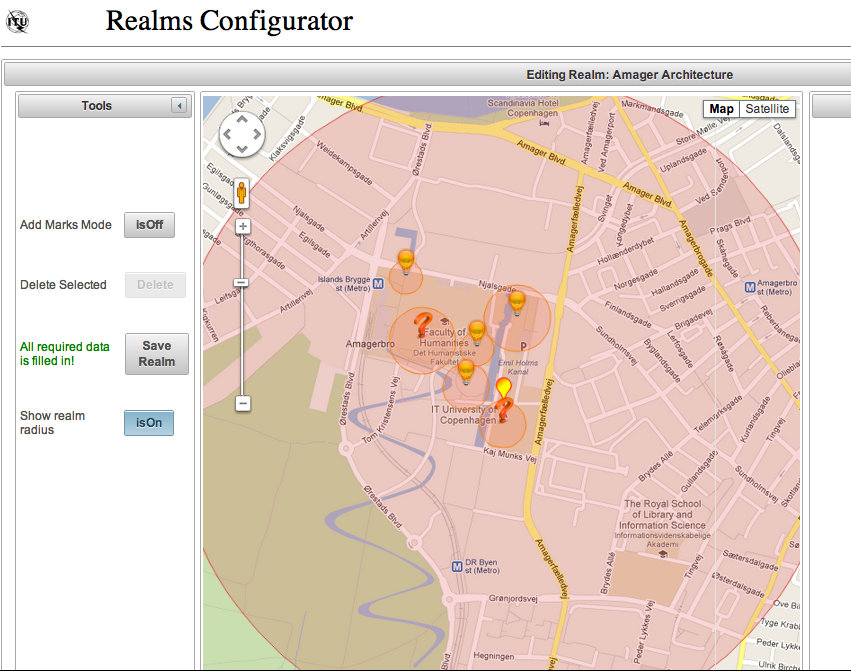
\includegraphics[width=0.8\linewidth]{fig/amager_configuration}
	\caption{Configuration for the test Realm Amager Architecture}
	\label{fig.amager.arc}
\end{figure}

\noinden We asked the participants to take a walk we us outside the university to play the scenario. The users were given a smartphone with the installed mobile application and GPS, Wifi and mobile data connection turned on. They were told that a Realm They were also told in which direction to walk without telling them which buildings in that direction that were marked. We kept walking around until at least 3 marks had been discovered after which the participants were told that we could go back or continue around to find a few more marks if they preferred.
\\\\
In the next section we discuss the results of the evaluation.

% subsection android_application_evaluation (end)
\clearpage
\section{Discussion} % (fold)
\label{sec:discusion}
In this section we discuss the evaluation results. 
\\\\
The main thing to note before we go in to discussing the evaluation results is, that the general level of programming experience for all our participants was high. As one of the objectives of the system was to bring end-user programming of location based systems to people without programming experience we will not conclude on this matter. We do however believe that the results of the evaluation provide good guidelines for future work on the system. 

\subsection{Usefulness} % (fold)
\label{sub:usefulness}
One of the main objectives of our evaluation was to investigate if users found our system useful. When abstracting the creating of augmented locations to a configuration level, a lot of expressiveness id lost. In our system users could only annotate locations with information or a question. These could then be explored through the mobile phone.
\\\\
All participants in our test however agreed that the system was indeed useful. We received a lot of suggestions for future features, but the basics of just putting information at a location was seen as a first useful way of presenting a system. One of our concerns with our approach was if the limited set of features would create a system that users did not find useful, but the feedback from the test participants leads us to believe that we have taken a right track.
% subsection usefulness (end)

\subsection{Usability} % (fold)
\label{sub:usability}
All participants were positive about the usability of the system. The use of Google maps to help users create Realms and marks was especially well received. The configurator did however suffer from small usability errors that should be improved. One thing we noticed during the test was that users rarely configured the radius of marks. While it seemed obvious to users to play around with the radius of the Realm, they rarely did so with marks. This was also pointed out by a single participant who suggested that marks had no initial radius to force users to think about how big it should be. As the sizes of marks and Realms play a large role in our thoughts of the system, we should consider how to get users to think about the size of marks.
\\\\
The usability of the mobile client was also well received, however as some participants pointed out, the functionality was very limited and so it was hard to not find it usable.
\\\\
All in all the system as a whole was found very ease to use. This leads us to believe that we have taken the right track by using Google maps and a web-interface that relies on text-boxes and buttons.
% subsection usability (end)

\subsection{Features} % (fold)
\label{sub:features}
The most requested feature was for the server to be able to push information to the client. Our current implementation has an update button that users can touch to query the server for any marks they are inside. All participants in the study requested this feature which leads us to prioritize this in our future work on the system. These two types of communication between server and client is what we refer to as communication type in our analysis section (see sec \ref{communication.type}) One of our original ideas behind making a pull-based system was enhance the feeling of a discovery service where users would walk around, hitting update to see if they found anything. However, as most participants pointed out, walking around with the phone in your hand can be quite annoying.
\\\\
The second most requested feature was some visual feedback on the client regarding the placement of realms and marks. Our idea with not providing any hints as to where to look for marks was to have an exploratory feeling to the system; users should go around the realm and explore it. However almost all participants requested some hints such as a map or textual hints.  
\\\\
The third most requested feature was to allow for more mark types. The two existing types - information and questions - were seen as a good start but to make it more interesting more should be added. Especially mark types that required more interaction between user and system was requested. One user also noted that it would be smart if programmers could write their own marks. This way the simplicity of the system would be preserved - as non programmers could use any existing marks - while experts could write their own. This is indeed a very interesting thought, though it would require a lot of work.
\\\\
Finally two users requested an augmented reality feature. It would indeed to be very interesting if users could use a wide variety of sensors in their phone - like camera and compass - to explore realms.
% subsection features (end)

\subsection{Realms} % (fold)
\label{sub:realms}
When we designed the system we came up with the name of Realms to describe an digitally augmented physical location. We thought of this metaphor as our system should allow user to enter new worlds where other rules might exist. We wanted to investigate how metaphor was perceived by others, so we during our evaluation interviews we asked them about the name and how it related to their experience of the system.
Most of the participants answered that they immediately though of computer games when they heard the word. As one participant put it \emph{"I though it would be a game or something entertaining"}. Only two participants thought the metaphor was good and this leads us to believe that we should either come up with a new metaphor or think about how we can communicate our thoughts behind it. 
% subsection realms (end)
\\\\
All in all the participants of our user study were very positive about our system. The system was fond useful and was easy to use and all participants believed that it was an interesting approach to location-based apps. The most requested features regarded visual feedback on the mobile client to help locate realms and marks. Furthermore we might need to reconsider the name Realms as it was mostly associated with computer games. 

\subsection{Comparison to existing systems} % (fold)
\label{sub:comparison_to_existing_systems}
Here we will look at some of the works on location systems described in the related works and discuss to what extend they could be implemented using Realms instead.
% subsection comparison_to_existing_systems (end)
% section discusion (end)
\clearpage
\section{Conclusions}
\label{sec.conclusions}


%\cleardoublepage
%\appendix

\clearpage

\nocite{*}
\bibliographystyle{plain}
\bibliography{bibliography}

\end{document}